\section{Ekvationer}

Om inte annat specifieras, kommer alla ekvationer följa symbolkonvention enligt denna tabellen.

\begin{table}[!h]
	\centering
	\begin{tabular}{| l | c |}
		\hline
		\textbf{Storhet} & \multicolumn{1}{|l|}{\textbf{Symbol}}\\
		\hline
		Tryck           & $p$ \\
		\hline
		Volym           & $V$ \\
		\hline
		Temperatur      & $T$ \\
		\hline
		Antal partiklar & $N$ \\
		\hline
		Antal mol       & $\nu$ \\
		\hline
		Inre energi     & $U$ \\
		\hline
		Värme           & $Q$ \\
		\hline
		Arbete          & $W$ \\
		\hline
	\end{tabular}
\end{table}

\twocolumn

\subsection{Allmänna ekvationer}

\paragraph{Konversion mellan $m$, $\nu$ och $N$}
\begin{align*}
	\nu = \frac{m}{M} = \frac{N}{N_\text{A}}.
\end{align*}
$M$ är gasens molara massa, massan per mol partiklar. Flera relationer kan härledas vid att använda $R = N_\text{A}k$.

\paragraph{Täthet}
\begin{align*}
	\rho = \frac{m}{V}
\end{align*}
Tätheten av en substans kan även definieras som
\begin{align*}
	n = \frac{N}{V}.
\end{align*}

\subsection{Termodynamikens huvudsatser}

\paragraph{Första huvudsatsen}
\begin{align*}
	\dd{U} = \idd{Q} - \idd{W}
\end{align*}
Vid att definiera första huvudsatsen så, definieras arbete gjort på systemet implisitt som positivt. Arbetet ges av
\begin{align*}
	\idd{W} = -p\dd{V}
\end{align*}

\paragraph{Andra huvudsatsen}
\begin{align*}
	\dd{S} = \frac{\idd{Q}}{T} \geq 0
\end{align*}
Likheten gäller för reversibla processer, och olikheten gäller för andra processer.

\paragraph{Tredje huvudsatsen}
\begin{align*}
	S(T = 0) = 0
\end{align*}

\subsection{Potensialer, derivator och annat diverse}

\paragraph{Inre energiens differensial}
Vid att kombinera termodynamikens första och andra huvudsats får man
\begin{align*}
	\dd{U} = T\dd{S} - p\dd{V}
\end{align*}

\paragraph{Fri energi}
\begin{align*}
	& F = U -TS\\
	& \dd{F} = -S\dd{T} - p\dd{V}
\end{align*}
Vid isoterma processer är $\idd{W} = \dd{F}$.

\paragraph{Entalpi}
\begin{align*}
	& H = U + pV \\
	& \dd{H} = T\dd{S} + V\dd{p}
\end{align*}

Ej kontinuerlig vid fasövergång.

\paragraph{Fri entalpi}
\begin{align*}
	& G = H - TS \\	
	& \dd{G} = -S\dd{T} + V \dd{p}
\end{align*}

Kontinuerlig vid fasövergång.

\paragraph{Uppvärming av ett ämne}
\begin{align*}
	\idd{Q} = mc\dd{T}
\end{align*}
$c$ är ämnets specifika värmekapacitet.

\paragraph{Molara värmekapaciteter}
När man värmer upp ett ämne, ger värmekapaciteten information om hur mycke temperaturen ökar när en given mängd värme tillförs. Den molara värmekapaciteten är värmekapaciteten per stoffmängd av ämnet, och är den samma för samma substansen. Molara värmekapaciteter är definierade som
\begin{align*}
	C_V = \frac{1}{\nu}\left(\pdv{U}{T}\right)_V, \\
	C_p = \frac{1}{\nu}\left(\pdv{H}{T}\right)_p.
\end{align*}
$C_V$ är den molara värmekapaciteten när värme tillförs vid konstant colym, och $C_p$ är den molara värmekapaciteten när värme tillförs vid konstant tryck.

\paragraph{Utvidgning}
Kroppar kan utvidga sig vid ändringar i omgivningarna. Utvidgningen relativt till originalvolymen kan kvantiseras vid att definiera relativa utvidgningskoefficienter som
\begin{align*}
	\kappa = -\frac{1}{V}\left(\pdv{V}{P}\right)_T, \\
	\alpha_V = -\frac{1}{V}\left(\pdv{V}{T}\right)_P.
\end{align*}
Vid att addera sådana ändringar kan man få den totala relativa volymändringen vid en given process enligt
\begin{align*}
	\frac{\dd{V}}{V} = -\kappa\dd{p} + \alpha_V \dd{T}
\end{align*}

\paragraph{Molar värmekapacitet för fasta ämnen}
\begin{align*}
	C = 3R
\end{align*}

\paragraph{Mikroskopisk entropi}
Ett system i ett givet makrotillstånd, definierad av termodynamiska storleker som tryck och temperatur, har en visas multiplicitet $W$ associerad med det givna makrotillståndet. Mutlipliciteten är antalet möjliga tillstånd partiklerna i systemet kan befinna sig så att systemet fortfarande karakteriseras av dom samma termodynamiska  storlekerna. Multipliciteten är kopplad till entropien vid Boltzmanns lag,
\begin{align*}
	S = k\ln{W}
\end{align*}

\subsection{Gaser}

\paragraph{Tillstånd}

\paragraph{Ideala gaslagen}
\begin{align*}
	pV = \nu RT = NkT.
\end{align*}
$N$ är antalet partiklar i gasen och $\nu$ är antalet mol partiklar i gasen.

\paragraph{van der Waals' tillståndsekvation}
\begin{align*}
	p = \frac{NkT}{V - Nb} - a\left(\frac{N}{V}\right)^2\\
	\left(p + \frac{a_0}{v^2}\right)(v - b_0) = RT
\end{align*}
Dessa är båda ekvivalenta versioner av van der Waals' tillståndsekvation, var man introduserar $a_0 = a N_\text{A}^2$, $b_0 = bN_\text{A}$ och $v = \frac{V}{\nu}$. $a$ innehåller information om växelverkan mellan partiklarna och $b$ innehåller information om partiklarnas volym.

\paragraph{Maxwell-Boltzmann-fördelingen}
Partiklarna i en ideal gas har olik fart. Antalet partiklar med en given fart $v$ per volym är fördelad enligt
\begin{align*}
	n(v) = Cv^2e^{-\frac{mv^2}{2kT}},
\end{align*}
var $m$ är en partikels massa. Vi krävjer att fördelingen är normaliserad, dvs.
\begin{align*}
	\int_0^{\infty}\dd{v}n(v) = \frac{N}{V},
\end{align*}
som ger
\begin{align*}
	K = 4\pi n \left(\frac{m}{2\pi kT}\right)^\frac{3}{2}.
\end{align*}
Från detta kan man räkna ut en mest sannolik fart $v_\text{p}$, en förväntad fart $<v>$ och en RMS-fart $v_\text{RMS}$. Dessa är
\begin{align*}
	& v_\text{p} = \sqrt{\frac{2kT}{m}}\\
	& \expval{v} = \sqrt{\frac{8kT}{\pi m}}\\
	& v_\text{p} = \sqrt{\expval{v^2}} = \sqrt{\frac{3kT}{m}}.
\end{align*}
Man kan även räkna ut en medelenergi per partikel, som är
\begin{align*}
	\expval{E} = \frac{n}{2}kT,
\end{align*}
var $n$ är antalet kvadratiska frihetsgrader per partikel. För en enatomig ideal gas är det
\begin{align*}
	\expval{E} = \frac{3kT}{2}.
\end{align*}
Det följer även att
\begin{align*}
	& U = NE = N\frac{n}{2}kT\\
	& pV = \frac{2}{n}U
\end{align*}

\paragraph{Medelfri väg}
Medelavståndet mellan två kollisioner i en ideal gas är
\begin{align*}
	l = \frac{kT}{p\pi d^2\sqrt{2}} = \frac{1}{n\pi d^2\sqrt{2}}
\end{align*}
var $n$ är partikeltätheten och $d$ är partiklernas diameter.

\paragraph{Stöttal}
Stöttalet är antalet partikler som kolliderar med en yta per enhet area och tid, och fås som
\begin{align*}
	\nu * = \frac{1}{4}n\expval{v} = \frac{p}{\sqrt{2\pi mkT}}
\end{align*}
var $n$ är partikeltätheten.

\paragraph{Molara värmekapaciteter för ideala gaser}
Vid att använda definitionerna av molara värmekapaciteter och uttrycket för indra energin till en ideal gas kan man visa att den molara värmekapaciteten är
\begin{align*}
	C_V = \frac{3}{2}R
\end{align*}
för en enatomig gas,
\begin{align*}
	C_V = \frac{5}{2}R
\end{align*}
för en tvåatomig gas och
\begin{align*}
	C_V = \frac{n}{2}R
\end{align*}
för en gas var partiklerna har $n$ kvadratiska frihetsgrader. Man kan även visa att generelt för ideala gaser är
\begin{align*}
	C_p = C_V + R
\end{align*}

\subsection{Adiabater och Carnotprocesser}

\paragraph{$pV$-representation av adiabatiska processer}
För reversibla adiabatiska processer gäller att $\idd{Q} = 0$. Detta implicerar att
\begin{align*}
	& pV^\gamma = c_1, \\
	& TV^{\gamma - 1} = c_2, \\
	& Tp^{\frac{1-\gamma}{\gamma}} = c_3, \\
\end{align*}
var alla $c_i$ är olika konstanter och $\gamma$ ges av
\begin{align*}
	\gamma = \frac{C_p}{C_V}
\end{align*}

\paragraph{Carnotprocesser}
I en Carnotprocess opereras det mellan två reservoarer med olika temperaturer. Kretsprocessen består av två isotermer a och c, samt två adiabater b och d, som illustrerad i figur \ref{fig:carnot_cycle}.
\begin{figure}[!ht]
	\centering
	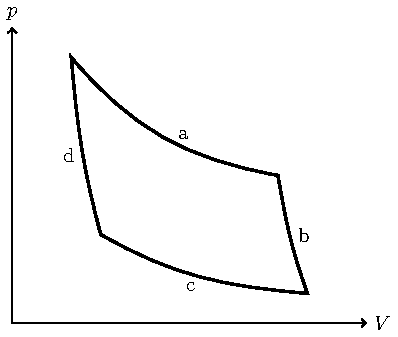
\includegraphics[width = \linewidth]{./Images/carnot/carnot.pdf}
	\caption{Carnotprocess i ett $pV$-diagram.}
	\label{fig:carnot_cycle}
\end{figure}

\paragraph{Carnotmaskiner}

Vi betraktar tre olika sorter Carnotmaskiner:
\begin{itemize}
	\item värmemaskiner, som använder värme till att göra ett arbete
	\item värmepumpar, som använder arbete till att värma upp ett reservoar
	\item kylmaskiner, som använder arbete till att kyla ned ett reservoar
\end{itemize}
Om processen körs medurs, avger den värma reservoaren värmen $Q_\text{H}$ vid temperatur $T_\text{H}$, medan den kalla reservoaren tar upp värmen $Q_\text{L}$ vid temperaturen $T_\text{L}$. Maskinen gör då arbetet $-W$. För en Carnotprocess kan man då visa att
\begin{align*}
	& \frac{Q_\text{H}}{T_\text{H}} = \frac{Q_\text{L}}{T_\text{L}}, \\
 	& W = Q_\text{H} - Q_\text{L}.
\end{align*}

\paragraph{Carnotmaskiners verkningsgrad}
Om man definierar en verkningsgrad $\eta$ som
\begin{align*}
	\eta = \frac{\text{Nyttig energi}}{\text{Energi vi putter in}}
\end{align*}
kan man visa följande verkningsgrader för Carnotprocesser:
\begin{itemize}
	\item Värmemaskin: $\eta = \frac{W}{Q_\text{H}} = \frac{T_\text{H} - T_\text{L}}{T_\text{H}}$
	\item Värmepump: $\eta = \frac{Q_\text{H}}{Q_\text{W}} = \frac{T_\text{H}}{T_\text{H} - T_\text{L}}$
	\item Kylmaskin: $\eta = \frac{Q_\text{L}}{W} = \frac{T_\text{L}}{T_\text{H} - T_\text{L}}$
\end{itemize}

\subsection{Värmetransport}

I denna sektion kommer olika mekanismer för värmeflöde att diskuteras. Vid termisk jämvikt är alla flöden $0$, medan vid stationära betingelser är alla flöden lika och konstanta med avseende på tid.

\subsubsection{Värmeledning}

\paragraph{Värmeledning genom ett fast ämne}
Värmeflödet $\Phi$ är givet av
\begin{align*}
	\Phi = \frac{\lambda}{d}A(T_\text{i} - T_\text{y}),
\end{align*}
var $\lambda$ är ämnets värmeledningsförmåga, $d$ är tjockleken och $T_\text{i}, T_\text{y}$ är temperaturen på varje sida av ämnet. Man kan även definiera ett värmeflödet per area $\phi = \frac{\Phi}{A}$.

Vid att definiera en värmeledning $U = \frac{\lambda}{d}$, kan man skriva
\begin{align*}
	\Phi = UA(T_\text{i} - T_\text{y}),
\end{align*}
analogt med i elläran. I denna analogien representerar $\Phi$ strömmen, $T_\text{i} - T_\text{y}$ spänningen och $\frac{1}{UA}$ motståndet. Vi definierar därför värmemotståndet $R = \frac{1}{U}$.

\paragraph{Värmeledning via gas}
Om ett fast ämne med temperatur $T_2$ är i kontakt med en gas med temperatur $T_1 > T_2$, är värmeflödet från gasen till det faste ämnet
\begin{align*}
	\Phi = \alpha A(T_1 - T_2).
\end{align*}
Igen definierar vi värmemotståndet $R = \frac{1}{\alpha}$.

\paragraph{Värmeledning genom flera föremål}
Om det sker värmeledning genom flera föremål, kan man räkna ut (medel)värmeflödet vid att använda temperaturerna på varje sida, samt det totala värmemotståndet, analogt med i dom två tidligare fallen. Det totala värmemotståndet, analogt med elläran, är
\begin{align*}
	R = \sum R_i,
\end{align*}
var summan göras över alla föremål.

\subsubsection{Strålning}
En svart kropp är en kropp som absorberar all inkommande strålning. I slika kroppar skapas elektromagnetiska vågor med alla mögliga frekvenser. För att analysera hur mycke energi svarta kroppar strålar ut, måste man först förstå hur mycke energi dom har lagrad i sig.

\paragraph{Elektromagnetisk strålning}
Elektromagnetiska vågor karakteriseras av en frekvens $\nu$ och en våglängd $\lambda$, som uppfyllar sambandet
\begin{align*}
	c = \nu\lambda.
\end{align*}
Strålningen transporteras av enskilda partikler som kallas fotoner. Ett foton har energi
\begin{align*}
	E = h\nu.
\end{align*}

\paragraph{Plancks lag}
Den inra energien per volym är $u = \frac{U}{V}$. Dens spektraltäthet, $\pdv{u}{\nu}$, är
\begin{align*}
	\pdv{u}{\nu} = \frac{8\pi h\nu^3}{c^3}\frac{1}{e^{\frac{h\nu}{kT}} - 1}.
\end{align*}

\paragraph{Svarta kroppars inre strålningsenergi}
Vid att integrera Plancks lag kan man räkna ut inre energin som
\begin{align*}
	U = V\frac{\pi^5}{15}\frac{8h}{c^3}\left(\frac{kT}{h}\right)^4
\end{align*}

\paragraph{Stefan-Boltzmanns lag}
Vid att kombinera det man vet om strålningsenergi med kinetisk gasteori, var man betrakter strålningen i en svart kropp som en gas av fotoner, får man Stefan-Boltzmanns lag
\begin{align*}
	\Phi = \sigma AT^4,
\end{align*}
var $\sigma$ kan uttryckas med andra konstanter som
\begin{align*}
	\sigma = \frac{2\pi^5 k^4}{15c^2 h^3}.
\end{align*}

\paragraph{Extremvärden för svartkroppsstrålning}
Svartkroppsstrålning har maxima, båda med avseende på frekvens och våglängd. Dessa maxima inträffar inte samtidigt! Dom kan räknas ut som
\begin{align*}
	& \frac{h\nu_\text{max}}{kT} = 2.821, \\
	& \lambda_\text{max}T = \SI{2.898E-3}{\meter~\kelvin}.
\end{align*}

\paragraph{Strålning på en kropp}
Om en kropp träffs av strålning, kan strålningen antingen arbsorberas, reflekteras eller transmitteras. Sannolikheten för varje av dessa anges med sannolikhetsfaktorer, som generellt är frekvensavhengiga. För arbsorptionsfaktoren $\alpha$, reflektionsfaktoren $\rho$ och transmissionsfaktoren $\tau$ gäller sambandet
\begin{align*}
	\alpha + \rho + \tau = 1
\end{align*}

\paragraph{Kirchoffs lag}
En kropp har även en emissivitet $\varepsilon$, som anger hur effektivt ytan strålar ut termisk energi. För en svart kropp är denna $1$. För att termisk jämvikt ska vara möjligt för strålande kroppar, måste varje kropp ha
\begin{align*}
	\varepsilon = \alpha
\end{align*}